\chapter{Analiza wymagań}
\label{cha:inzyneriaWymagan}
Nadrzędnym celem tworzonych systemów informatycznych jest realizacja wymagań klienta. W przeciwnym razie końcowy użytkownik nie będzie zainteresowany ich odbiorem. Najważniejszą rzeczą we wstępnej fazie procesu tworzenia oprogramowania jest dbałość o zidentyfikowanie właściwych wymagań dla danego problemu.

\section{Zidentyfikowanie użytkowników aplikacji}
\label{sec:uzytkownicy}
Użytkownicy systemu mogą zostać podzielieni na dwie grupy:
\begin{itemize}
\item niezalogowanych
\item zalogowanych
\end{itemize}
System udostępnia pewne funkcjonalności osobom niezarejestrowanym w celu zachęcenia ich do korzystania z serwisu. Zezwolenie na używanie pewnych funkcjonalności serwisu wpływa bardzo pozytywnie na pierwsze wrażenie jakie odnosi użytkownik portalu. Bardzo często zdarza się, że osoba która nie może przetestować bez rejestracji czy serwis będzie odpowiadał jej potrzebom, nie będzie skłonna podać swoich danych osobowych.

\section{Wymagania funkcjonalne}
\label{sec:wymaganiaFunkcjonalne}
Analiza wymagań funkcjonalnych umożliwia zidentyfikowanie i opisanie pożądanego zachowania systemu. Zgodnie z jedną z definicji, wymaganie funkcjonalne to stwierdzenie, jakie usługi ma oferować system, jak ma reagować na określone dane wejściowe oraz jak ma się zachowywać w określonych sytuacjach. W niektórych wypadkach wymagania funkcjonalne określają, czego system nie powinien robić. Wymagania mogą również być ograniczeniem w procesie implementacji systemu.\cite{requirements}\\ Wymaganie funkcjonalne które zostały zidentyfikowane dla użytkowników niezalogowanych:
\begin{itemize}
\item System umożliwia zarejestrowanie się
\item System umożliwia zalogowanie się 
\item System umożliwia przeglądanie ofert
\item System umożliwia używanie filtrów
\end{itemize}
Wymaganie funkcjonalne, które zostały zidentyfikowane dla użytkowników zalogowanych:
\begin{itemize}
\item System umożliwia wylogowanie się
\item System umożliwia dodawanie ofert do obserwowanych
\item System umożliwia zapisanie filtrów
\item System umożliwa przeglądanie obserwowanych ofert
\item System umożliwa dodanie oferty 
\end{itemize}
System ponadto powinien:
\begin{itemize}
\item Periodyczne wyszukiwać spersonalizowane oferty dla użytkowników
\item Wysyłać maile do użytkowników z wynikami wyszukiwania
\item Zliczać odsłony oferty
\end{itemize}

\section{Wymagania niefunkcjonalne}
\label{sec:wymaganiaNiefunkcjonalne}
Analiza wymagań niefunkcjonalnych pozwala na określenie kryteriów, które będą brane pod uwagę przy ocenianiu poprawności działania danego systemu. \\
Wymaganie niefunkcjonalne które zostały określone dla omawianego systemu:
\begin{itemize}
\item System powinien być niezawodny
\item System powinien zwracać wyniki niemal natychmiast
\item System powinien umożliwiać dodawanie nowych języków
\item System powinien być bezpieczny
\item System powinien być intuicyjny w użytkowaniu
\end{itemize}

\section{Diagram przypadków użycia}
\label{sec:przypadkiUzycia}
\noindent
\begin{minipage}{\linewidth}
\makebox[\linewidth]{
  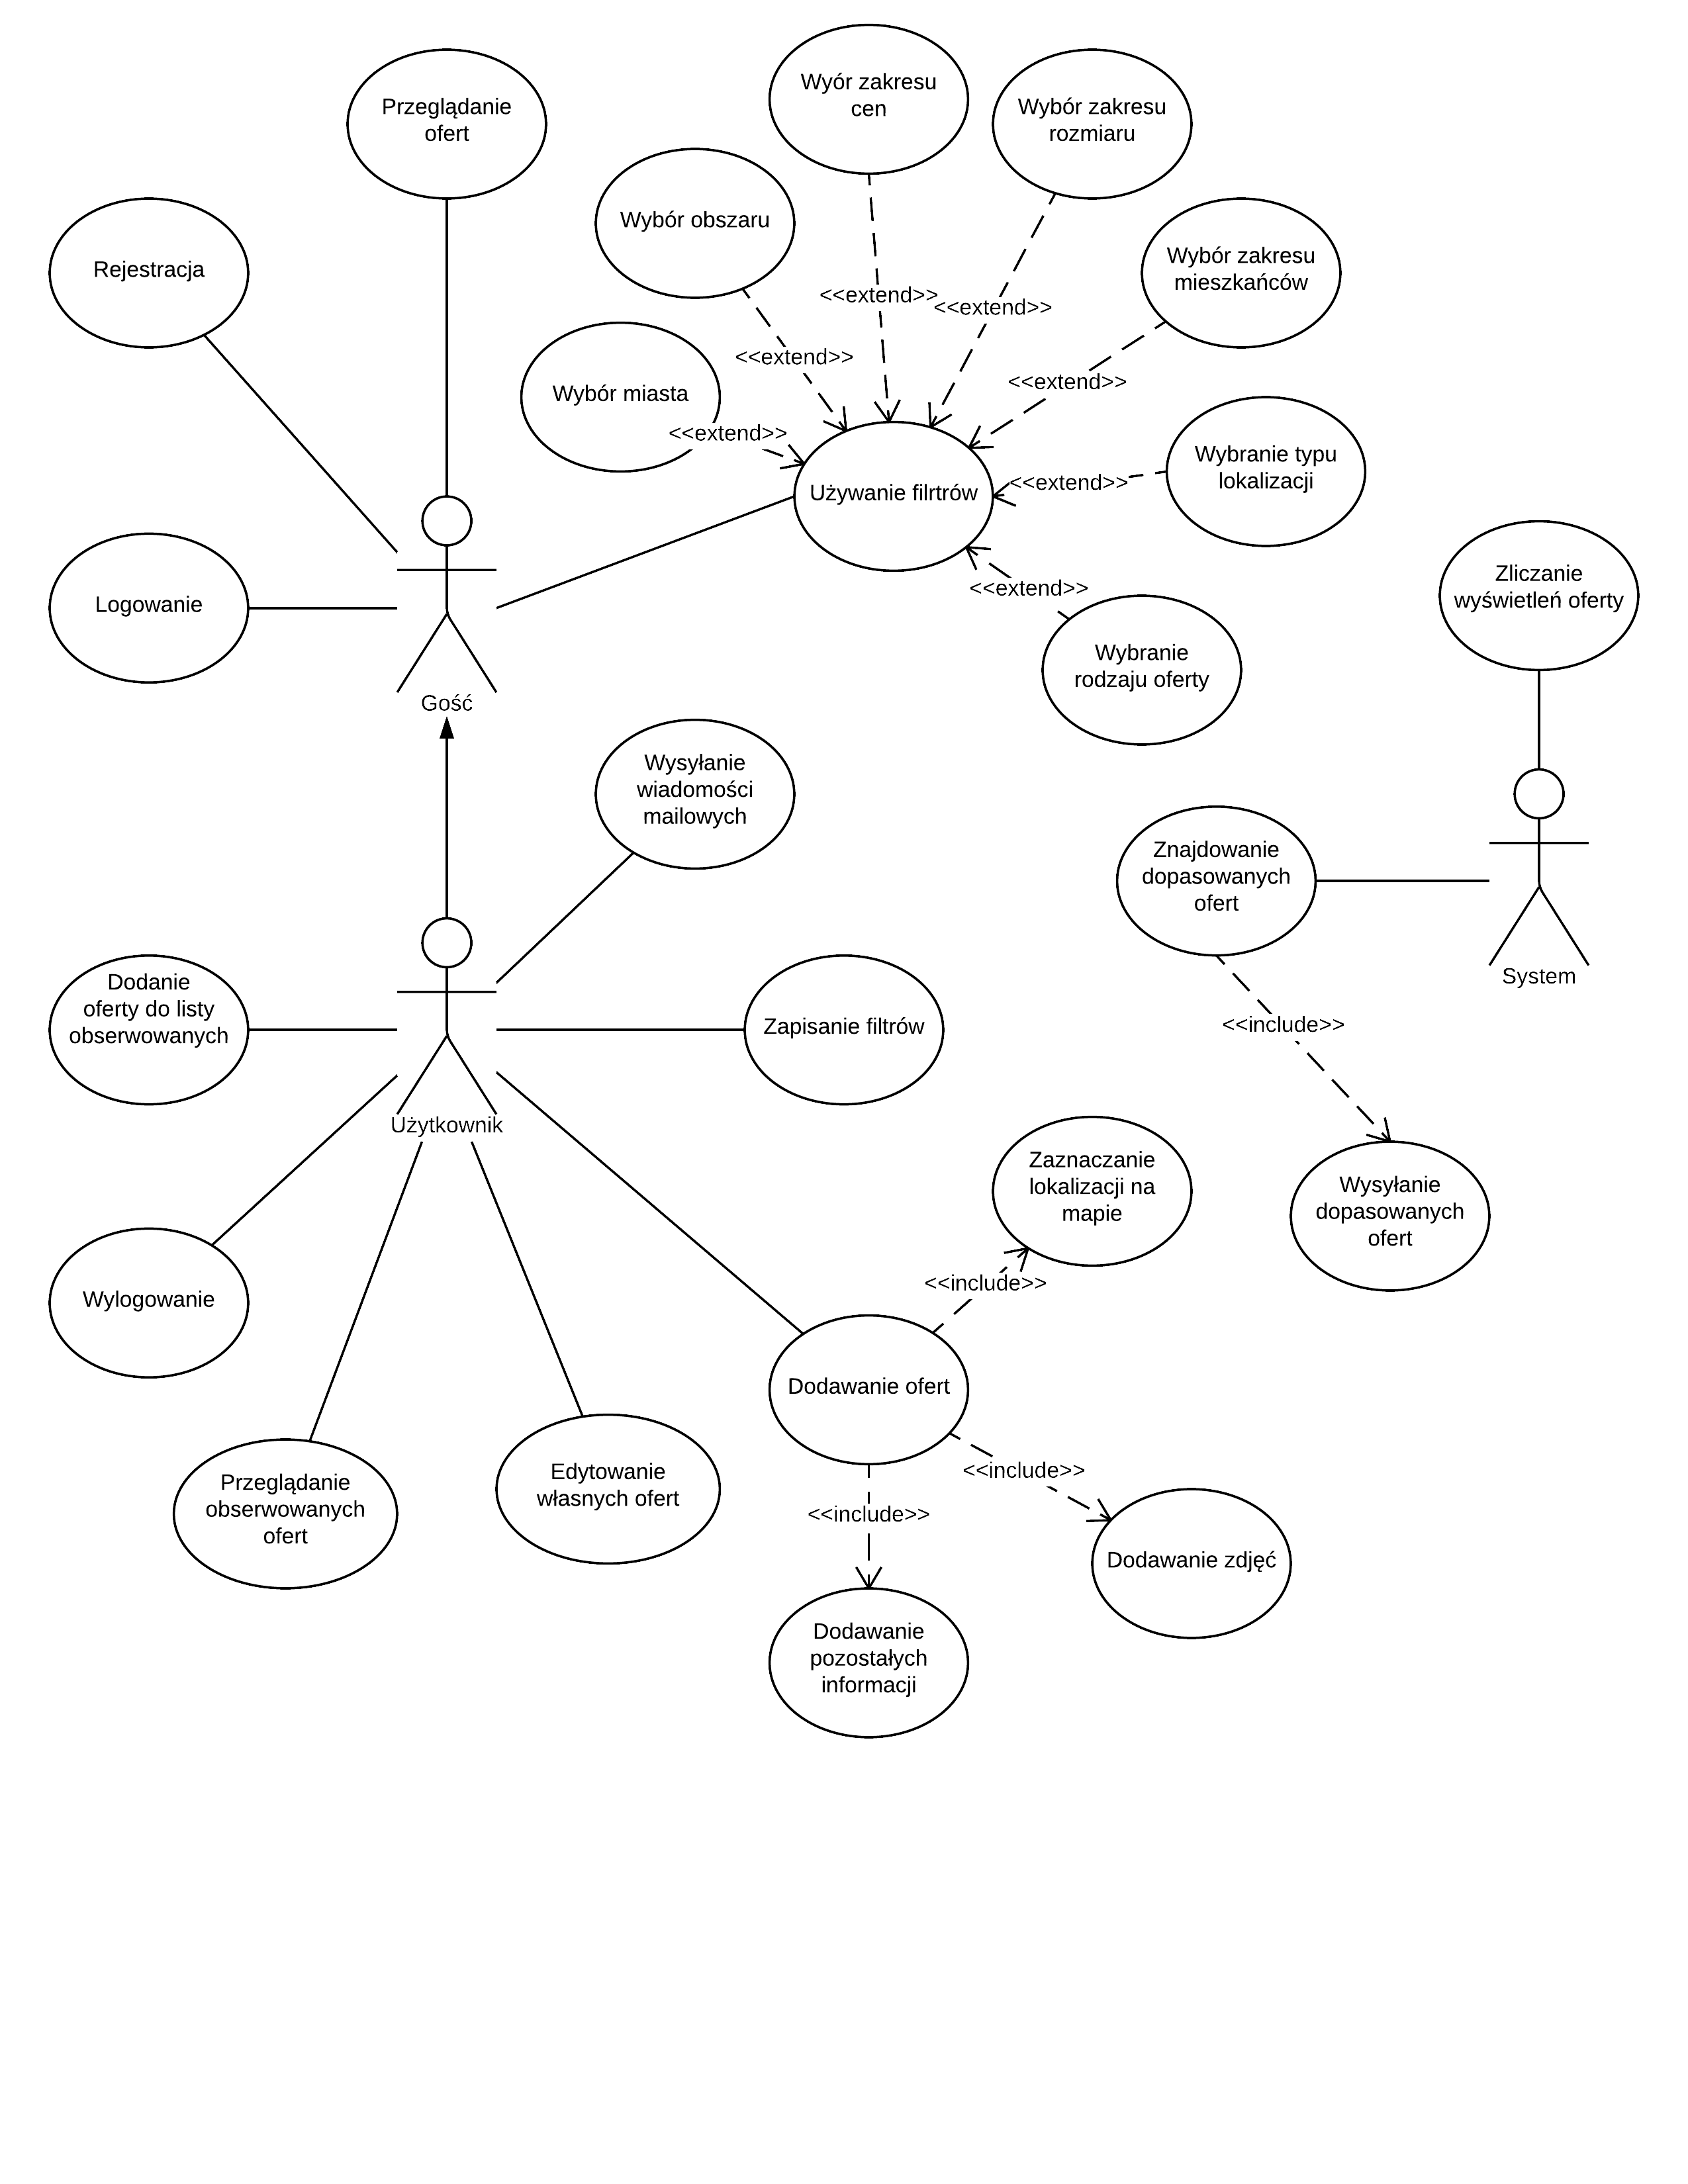
\includegraphics[keepaspectratio=true,scale=0.75]{pictures/use-case.png}}
\captionof{figure}{Diagram przypadków użycia}\label{use-case}
\end{minipage}

\section{Zidentyfikowanie obiektów świata rzeczywistego}
Poparawna identyfikacja obiektów świata rzeczywistego jest niezbędna do stworzenia poprawnego schematu bazy danych. Obiekty, które zostały zidentyfikowane podczas procesu analizy aplikacji to:
\begin{itemize}
\item Użytkownik (user)
\item Oferta (offer)
\item Zdjęcie (photo)
\item Lokalizacja (location)
\item Filtr (filter)
\end{itemize}
Zależności jakie zachodzą pomiędzy obiektami:\\
\noindent
\begin{minipage}{\linewidth}
\makebox[\linewidth]{
  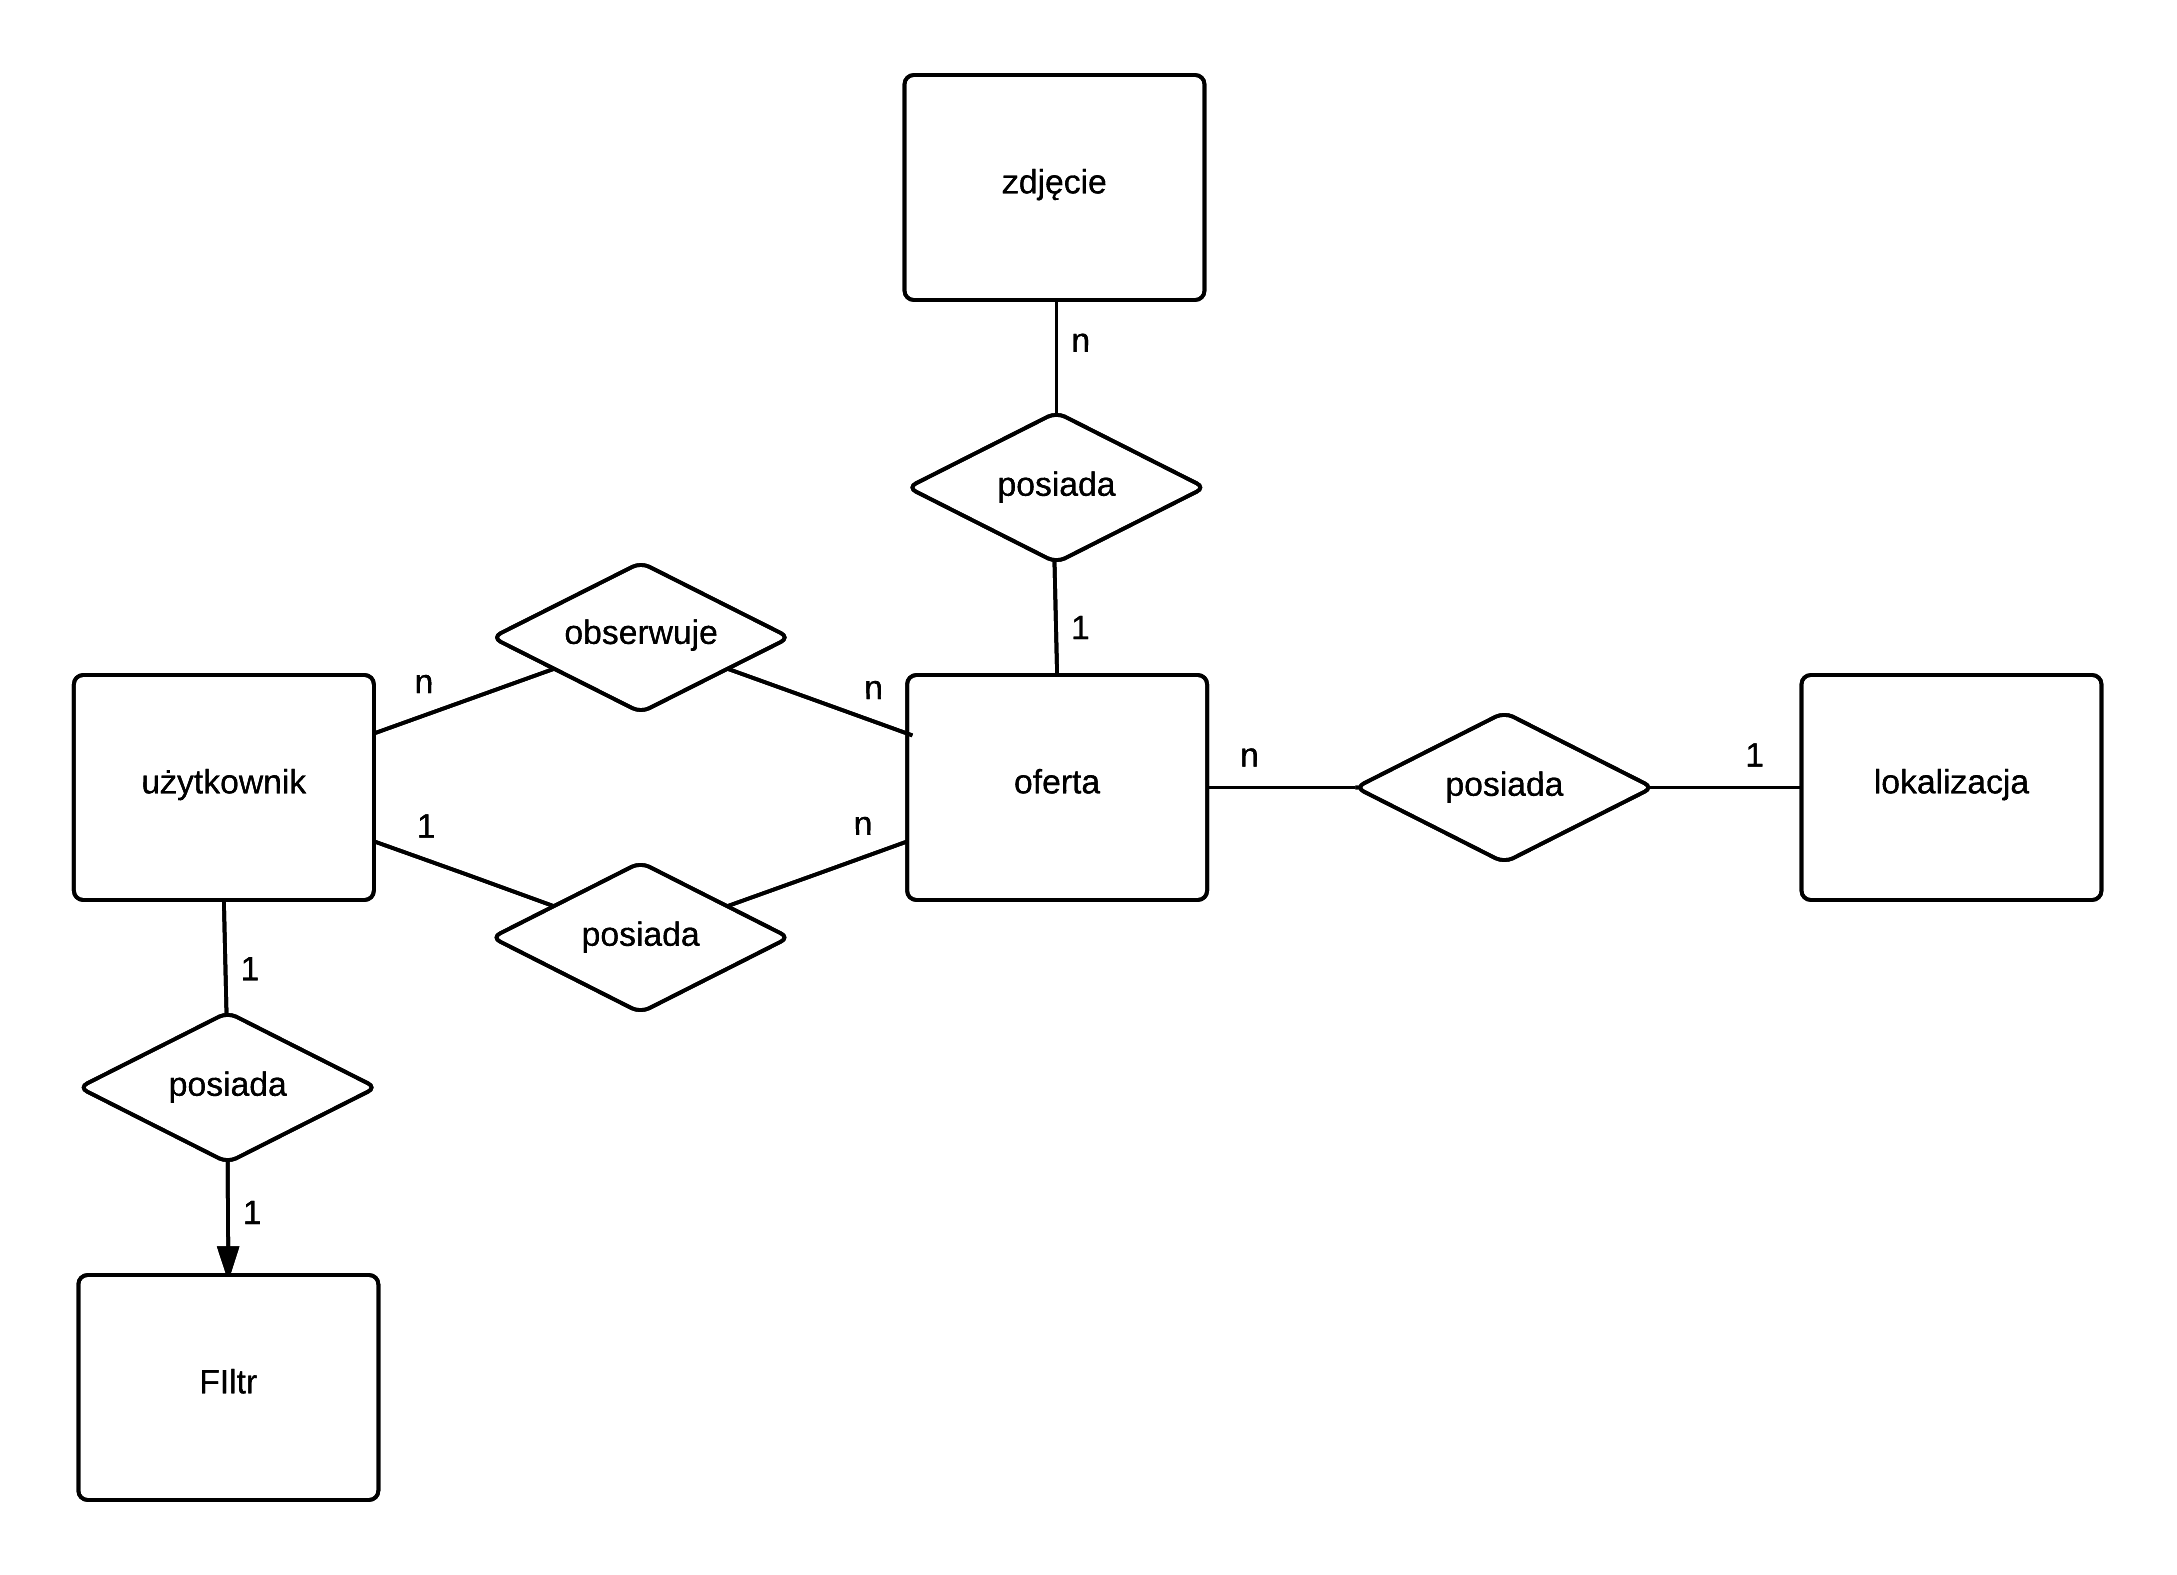
\includegraphics[keepaspectratio=true,scale=0.85]{pictures/erd.png}}
\captionof{figure}{Diagram ERD relacji pomiędzy encjami}\label{erd}
\end{minipage}
